
\section{Sistemi interconnessi - esteso}
È possibile suddividere un sistema comunque complesso, composto da più
sottosistemi che interagiscono tra loro.
Al fine di formalizzare correttamente i sistema interconnessi si presentano i
tre blocchi principali.

Il primo è il blocco sistema, rappresenta il modello di un sistema, disegnato
mediante un rettangolo, con le frecce in ingresso e in uscita si indicano le
variabili di ingresso e uscita.
$$
Y_f(s) = W(s)U(s)
$$
\begin{figure}[h]
\centering
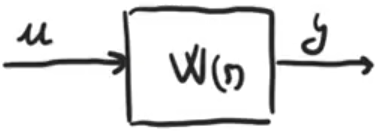
\includegraphics[width=0.3\linewidth]{blocco_sistema}
\end{figure}

Il secondo elemento è il nodo diramatore, ha un ingresso, poi con un punto
calcato si suddividono le uscite (nel dominio del tempo o di Laplace
$$
y_1(t) = y_2(t) = y_3(t) = u(t)
$$
\begin{figure}[h]
\centering
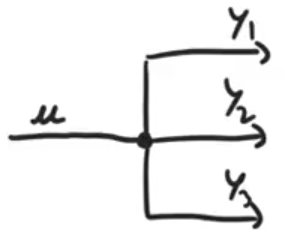
\includegraphics[width=0.3\linewidth]{blocco_nodo}
\end{figure}

\newpage
Il nodo sommatore invece, rappresentato mediante un cerchio o un quadrato
esegue somme o sottrazioni degli ingressi, fornendo una sola uscita
$$
y(t) = u_1(t) - u_2(t) + u_3(t)
$$
\begin{figure}[h]
 \centering
 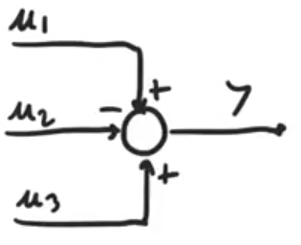
\includegraphics[width=0.3\linewidth]{blocco_sommatore}
\end{figure}

Per ottenere la rappresentazione di tutto il sistema è comodo operarne la sua
riduzione, per via algebrica o più comodamente per via grafica.
Le regole di riduzione si basano sulla presenza di tre connessioni canoniche,
in serie, in parallelo e in retroazione.

\subsection{Connessione in serie}
Due o più blocchi sono connessi in serie se l'ingresso del blocco
successivo coincide con l'uscita del precedente.
\begin{figure}[h]
\centering
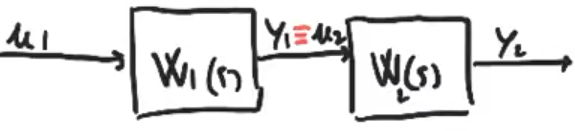
\includegraphics[width=\picwid]{blocchi_serie}
\end{figure}
Dal punto di vista sistemistico la serie può essere vista come un unico blocco
più grande con un'unica funzione di trasferimento $W(s)$ con ingresso $u$ e
uscita $y$.

Si ricava la riduzione, si presentano le relazioni algebriche dei due blocchi e
il vincolo topologico
$$\left\{\begin{aligned}
Y_1(s) &= W_1(s)U_1(s) \\
Y_2(s) &= W_2(s) U_2(s) \\
Y_1(s) &= U_2(s)
\end{aligned}\right.
\qquad
\begin{aligned}
Y(s) &= Y_2(s) = W_2(s)U_2(s) = W_2(s)Y_1(s) =\\
&=W_2(s)W_1(s)U_1(s) = W_2(s)W_1(s)U(s)
\end{aligned}$$
La funzione di trasferimento del blocco ridotto è dunque pari al prodotto delle
due funzioni di trasferimento dei sottosistemi.
Se il sistema è SISO la moltiplicazione è commutativa, non è vero per i sistemi
non SISO.

\newpage
\subsection{Connessione in parallelo}
Due o più sottosistemi sono connessi in parallelo se condividono lo stesso
ingresso, uscita di un nodo diramatore, e la loro uscita viene combinata in un
nodo sommatore.
\begin{figure}[h]
\centering
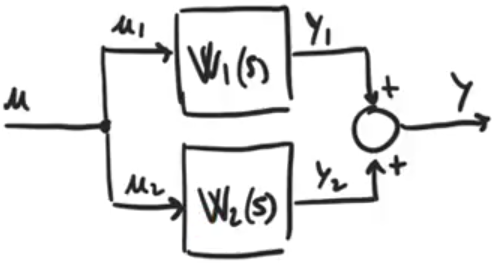
\includegraphics[width=\picwid]{blocchi_parallelo}
\end{figure}
Per ricavare l'unica funzione di trasferimento si procede in maniera analoga al
caso precedente, scrivendo le relazioni dei blocchi e dei due vincoli
sull'ingresso e l'uscita
$$
\left\{\begin{aligned}
Y_1(s) &= W_1(s) U_1(s) \\
Y_2(s) &= W_2(s) U_2(s) \\
U_1(s) &= U_2(s) = U(s) \\
Y(s) &= Y_1(s) + Y_2(s)
\end{aligned}\right.\qquad
\begin{aligned}
Y(s) & = Y_1(s) + Y_2(s) = W_1(s)U_1(s) + W_2(s) U_2(s) =\\
&=\left( W_1(s)+W_2(s)
\right) U(s)
\end{aligned}
$$
La funzione di trasferimento del blocco in parallelo è pari alla somma
algebrica delle rispettive funzioni di trasferimento dei sottosistemi.

\subsection{Connessione in retroazione}
Un sistema in retroazione è composto da due blocchi, il sistema $W_1$ che
genera l'uscita è chiamato \textit{catena di andata}, il blocco $W_2$ inferiore
prende il nome di \textit{catena di ritorno (o retroazione)} e chiude un anello
in cui ``girano'' le informazioni chiamato \textit{anello di retroazione}.
L'ingresso del sistema principale è dato dal confronto dell'ingresso $u$ di
riferimento e l'uscita $y_2$ del blocco di retroazione. Si può avere una
retroazione negativa o positiva a seconda del segno che compare nel blocco
sommatore in ingresso (quella in figura è negativa).

\begin{figure}[h]
\centering
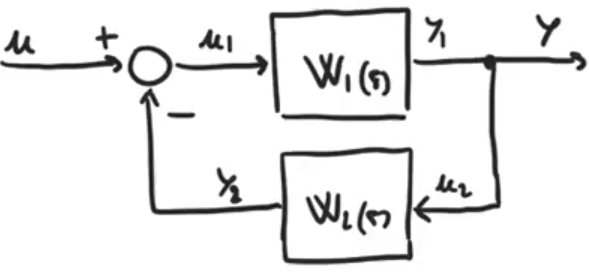
\includegraphics[width=\picwid]{blocchi_retroazione}
\end{figure}

Si analizzano le equazioni dei singoli blocchi e le due relazioni topologiche
$$
\left\{\begin{aligned}
Y_1(s) &= W_1(s) U_1(s) \\
Y_2(s) &= W_2(s) U_2(s) \\
U_1(s) &= U(s) - Y_2(s) \\
Y(s) &= U_2(s) = Y_1(s)
\end{aligned}\right.
$$

Sviluppando il sistema a partire dalla funzione in uscita si ricavano le due
funzioni di trasferimento per i sistemi in retroazione positiva e negativa
$$
\begin{aligned}
Y(s) & = W_1(s) U_1(s) = W_1(s) (U(s) - Y_2(s)) =\\
&=
W_1(s) (U(s) - W_2(s)U_2(s)) = W_1(s)(U(s)-W_2(s)Y(s)) \Rightarrow \\
&(1+W_1(s)W_2(s))Y(s) = W_1(s) U_1(s) \Rightarrow
Y(s) = \frac{W_1(s)}{1+W_1(s)W_2(s)}U(s)
\end{aligned}
$$
\begin{table}[h]
\centering
\begin{tabular}{c|c}
Retroazione negativa & Retroazione positiva \\
$W(s) = \frac{W_1(s)}{1+W_1(s)W_2(s)}$ &
$W(s) = \frac{W_1(s)}{1-W_1(s)W_2(s)}$
\end{tabular}
\end{table}

\subsubsection{Esempio non SISO}
Se il sistema non dovesse essere di tipo SISO come quello in esempio
$$
u=\begin{pmatrix}
u_1 \\ u_2
\end{pmatrix} \rightarrow
\begin{matrix}W(s)\\2\times2
\end{matrix}
\rightarrow y = \begin{pmatrix}
y_1 \\ y_2
\end{pmatrix}
$$
Sfruttando la sovrapposizione degli effetti si possono scomporre le uscite,
ogni termine può essere visto come la somma degli effetti di un singolo
ingresso alla volta, dunque per calcolare $y_1$ si studia la risposta ad $u_1$
quando $u_2$ è nulla e viceversa, poi si sommano i due contributi; analogamente
per $y_2$.
$$\left\{\begin{aligned}
Y_1 &= Y_1' + Y_1'' = W_{11}U_1 + W_{12}U_2\\
Y_2 & = Y_2' + Y_2'' = W_{21}U_1 + W_{22}U_2
\end{aligned}\right.$$

Dunque la $W(s)$ sarà
$$
W(s) = \begin{bmatrix}
W_{11}(s) & W_{12}(s) \\
W_{21}(s) & W_{22}(s)
\end{bmatrix}
$$
Da un punto di vista grafico saranno presenti quattro blocchi elementari
\begin{figure}[h]
\centering
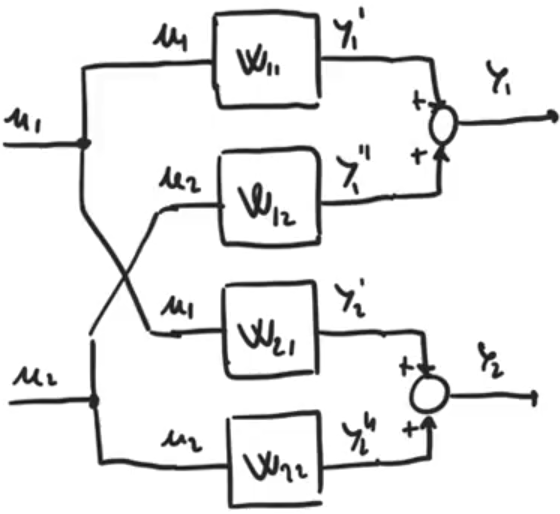
\includegraphics[width=\picwid]{blocchi_non_SISO}
\end{figure}

\subsection{Regole di elaborazione}
Può capitare che in una rete complessa non sia chiaro quali blocchi siano in
serie o in parallelo, potrebbe essere necessario eseguire delle
\textit{manovre} di spostamento dei blocchi che coincidono ad operazioni
algebriche che devono lasciare però inalterata la funzione di trasferimento
complessiva.
Durante queste operazioni è molto probabile che si perda il senso fisico delle
operazioni, l'importante è non variare la funzione di trasferimento.

Si supponga di avere la seguente condizione, per qualche motivo si vuole
spostare il blocco $W(s)$ a monte del nodo sommatore, sarà equivalente al
sistema formato da due blocchi.
\begin{figure}[h]
\centering
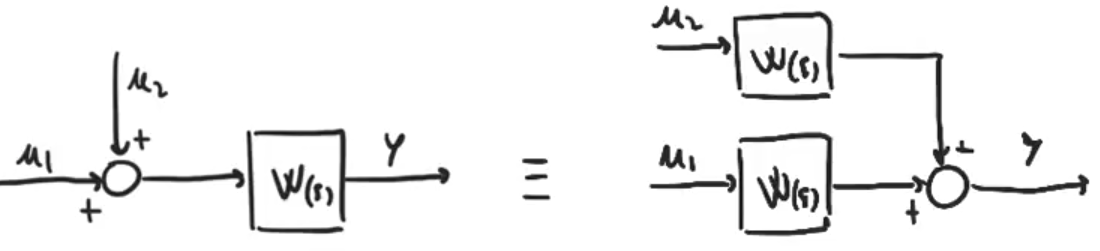
\includegraphics[width=0.7\linewidth]{blocchi_equivalenza_sommatore}
\end{figure}
Algebricamente si ottiene lo stesso risultato
$$
Y = W(U_1+U_2) \qquad \equiv \qquad Y= WU_1 + WU_2 = W(U_1+U_2)
$$
da un punto di vista fisico il sistema iniziale ha $n$ variabili di stato, il
secondo ha invece $2n$ variabili di stato, ma sono variabili ``fittizie'' e non
variabili fisiche.

Il caso duale è il seguente
\begin{figure}[h]
\centering
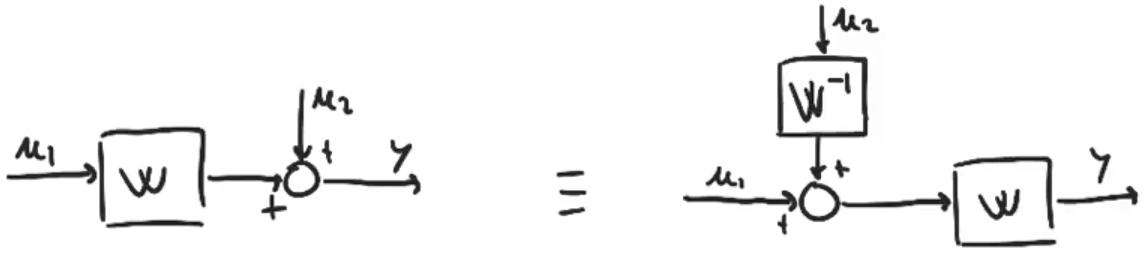
\includegraphics[width=0.7\linewidth]{blocchi_equivalenza_sommatore_a_valle}
\end{figure}
$$
Y = U_2 + WU_1 \qquad \equiv \qquad
Y = W(U_1 + W^{-1}U_2) = WU_1 + U_2
$$
51:00
